\chapter{Main Body}
\label{cha:Main Body}

\section{Trigger R\&D}
\label{sec:Trigger}
To trigger the counter of the WSB, there are a few possible solutions. The remote has to be wearable, and it has to be triggered during the game. This is hard to implement, because a usual button is too tiny to press during a game, and it can be frustrating to always aim for the trigger button. Therefore, I decided to use an accelerometer and count the points by simply tapping on the thigh. My idea is to mount the WSB remote on the inside of the thigh or as a knee pad replacement for example in volleyball. Then the vibrations/accelerations travel through the user's body and get measured by the WSB remote. But this can be rather hard, because during sports the body is always accelerating, and it could be hard to distinguish from a usual movement or a "thigh tip". If the accelerometer idea doesn't work out, I would use flexible membrane buttons to control the WSB. 

\subsection{Accelerometer R\&D}
\label{ssec:Accelerometer}
At my current lab at ETH I found an accelerometer to test out, if I can use it as a trigger.
\subsubsection{control LSM303C accelerometer}
Attention: Mind that the CS\_XL and CS\_MAG have to be pulled up to enable I\textsuperscript{2}C mode. and use external I\textsuperscript{2}C pullups, because on MKI163V1 devBoard are no pullup R's.

slave address: 0b00111010 = 0x3A \cite{DS_LSM303C}

\begin{figure}[H]
	\centering
	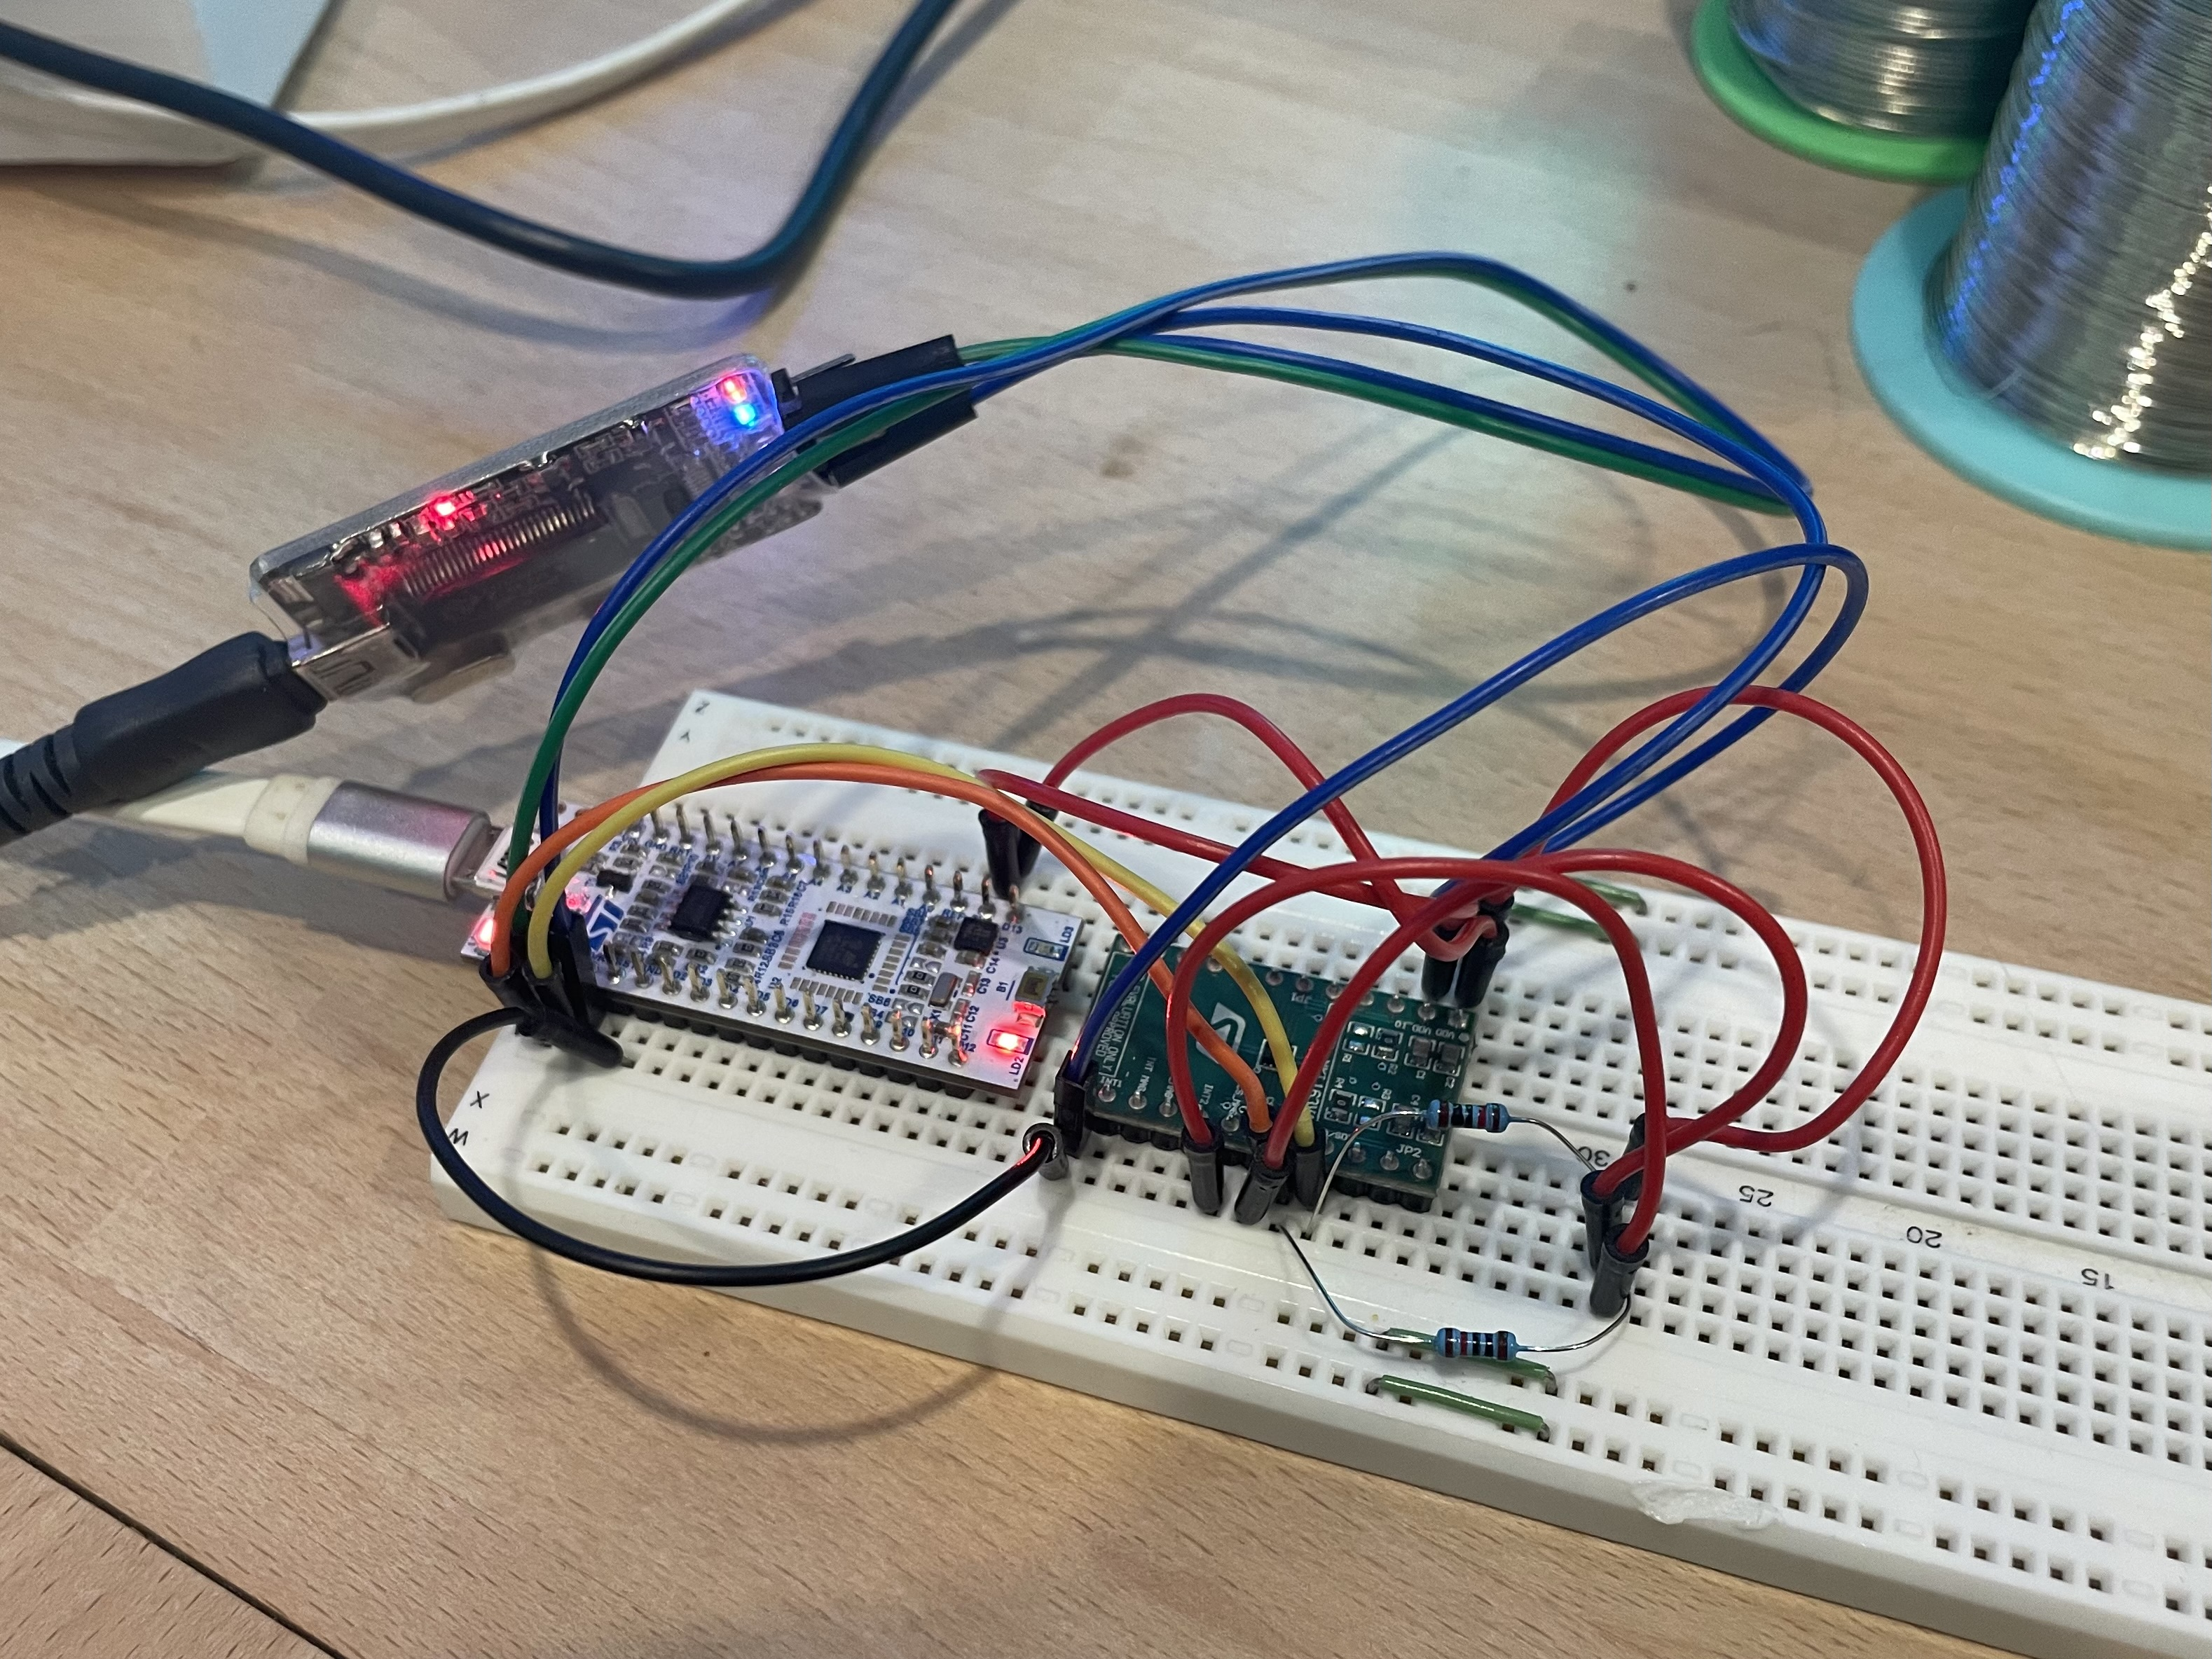
\includegraphics[width=10cm]{Resources/accTestLab.jpeg}
	\caption{Accelerometer test: setup}
	\label{fig:accTestLab}
\end{figure}

\subsubsection{First test the "WHO AM I" register}
Communication test: reg 0x0F should read as 0x41

\subsubsection{Read acceleration}
CTRL\_REG1\_A (0x20): 0x3F (Enable XYZ, 100Hz, block data overwriting)

CTRL\_REG2\_A (0x21): 0x00 (disable LPF)

CTRL\_REG3\_A (0x22): 0x00 (disable interrupts)

CTRL\_REG4\_A (0x23): 0x34 (enable I\textsuperscript{2}C, enable auto address increments, FS $\pm$8g)

CTRL\_REG5\_A (0x24): 0x00

CTRL\_REG6\_A (0x25): 0x00

CTRL\_REG7\_A (0x26): 0x00
\\

STATUS\_REG\_A (0x27):
Bit 3 set if xyz data is available / Bit 8 set if xyz data overrun.

OUT\_X\_L (0x28)(2bytes)   (0.061mg/LSB) @ FS=8g

OUT\_Y\_L (0x2A)(2bytes)   (0.061mg/LSB) @ FS=8g

OUT\_Z\_L (0x2C)(2bytes)   (0.061mg/LSB) @ FS=8g

\begin{figure}[H]
	\centering
	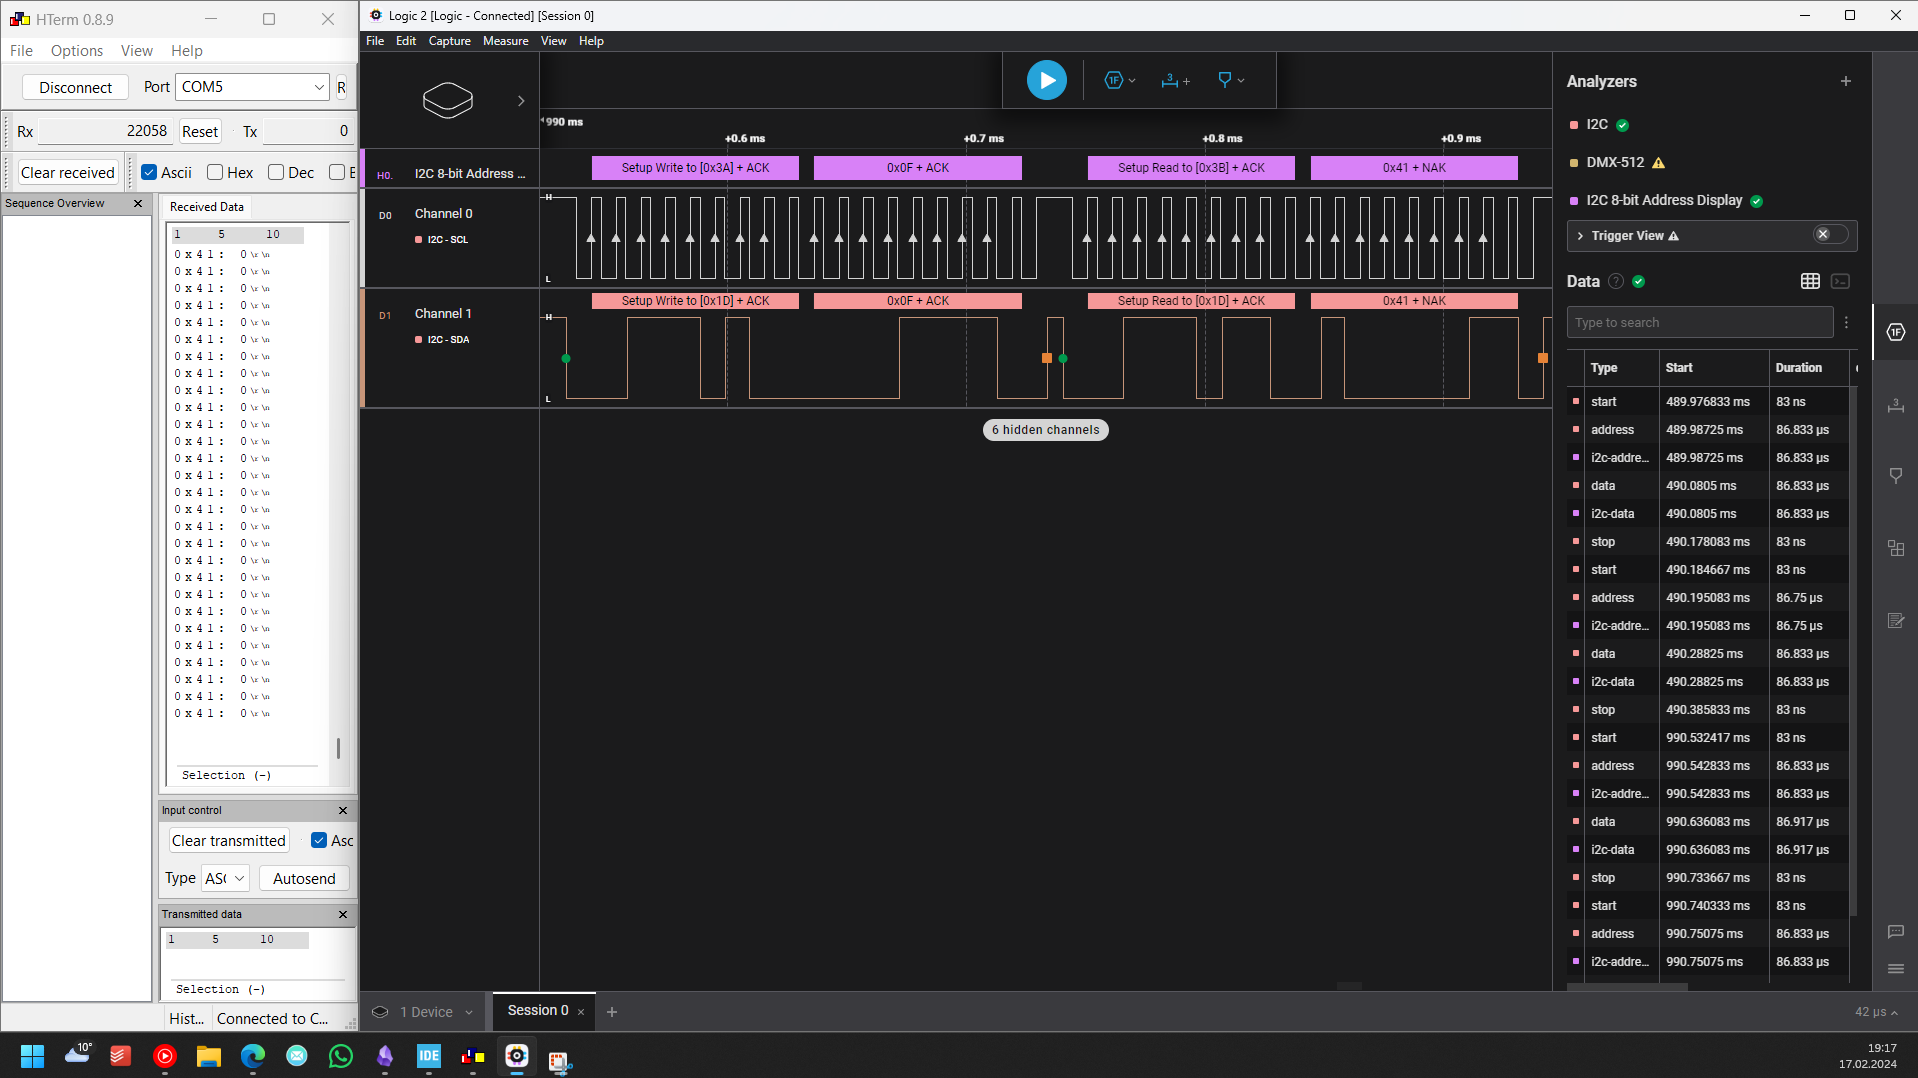
\includegraphics[width=17cm]{Resources/accTestLA.png}
	\caption{Accelerometer test: logic analyzer}
	\label{fig:accTestLA}
\end{figure}
\newpage

\subsubsection{Test Results}
After looking at the measurement results, I decided that it would be best to populate an accelerometer and the membrane buttons on the PCB, that I have an alternative if the accelerometer doesn't work out. Because it's hard to analyze if the accelerometer as trigger will work out during a game and I can't attach the current breadboard to my thigh to test the accelerometer out. But for the final design I'll probably choose the "STM LIS2HH12" accelerometer.

\begin{figure}[H]
	\centering
	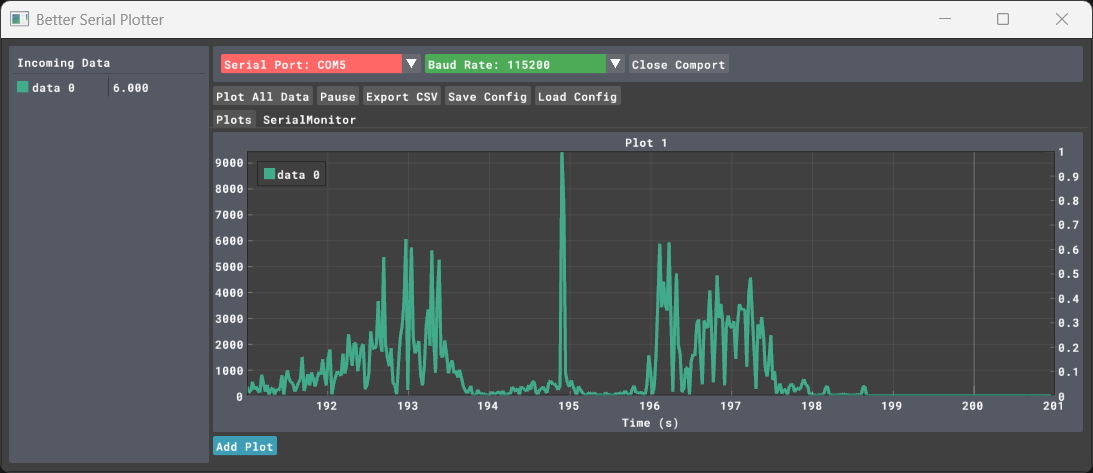
\includegraphics[width=17cm]{Resources/accTestMeas.png}
	\caption{Accelerometer test: results}
	\label{fig:accTestMeas}
\end{figure}

I hope that I can differentiate normal sports movement from "thigh taps" by looking at the momental acceleration. In Fig: \ref{fig:accTestMeas}, the middle pulse was a "thigh tap" and the first and last ones are movement from the body, which take a lot longer but don't peak out as high. The shown data is actually the variable "accDelta" from the "6\_Software/dev/LSM303C\_Test/Core/Src/ main.c" file.

\section{Battery Charging R\&D}
\label{sec:Battery Charging}
I'm sure, that I'll have to somehow power the WSB Remote as well as the WSB. Because they both have to be portable, I'm planning to use a rechargeable battery. For example Lithium Ion battery. And to use this battery I'll have to implement some protection circuits, as well as charging circuits. Important protection features are:
\begin{itemize}
    \item UVP - Under Voltage Protection (So the battery doesn't get broken)
    \item OVP - Over Voltage Protection (So the battery doesn't get broken)
    \item OTP - Over Temperature Protection (So the battery doesn't overheat or starts burning)
    \item OCP - Over Current Protection (So the circuits don't break)
\end{itemize}

So I started searching for LiIon charging ICs and I had looks at TIs ICs, like the "BQ25180YBGR" or "BQ25155YFPR". But the TI charging ICs are rather complicated and would take me too long to implement. Additionally after buying some samples of these ICs I recognized, that they are CSPs and really tiny, which makes them really hard to solder or make modifications on the PCB. So I got to my favourite semiconductor manufacturer STM and found the perfect IC, the STNS01. I also recognized, that STMs product portfolio is a lot smaller than TIs, which was quite overwhelming. STM only had about 5 ICs to choose from.


\section{Remote PCB}
\label{sec:Remote PCB}
The remote PCB connects all components together, such as the accelerometer, microcontroller and RF module. I decided to design a custom PCB and later order it, because there are too much and too small components to solder onto a development board. The WSBR PCB should have the following features according to the HW Concept. [\ref{sec:HW Concept}]

\begin{itemize}
    \item Battery charging through USB-C with battery level monitoring.
    \item Battery level monitoring when power button is pressed once.
    \item Start remote, when power button is pressed once and then again for longer.
    \item Flash MCU using USB-DFU mode when pressing the boot button.
    \item Use an accelerometer or three membrane buttons as a trigger to count points.
    \item Send data via RF (nRF24L01) to WSB and show the remote state with an RGB LED.
\end{itemize}


\subsection{Schematics}
The schematics were drawn using Altium Designer and are stored in the "5\_Hardware\\WSBR\_Board" directory. Full Schematics here: [\ref{fig:Remote Schematics}]

\label{ssec:Schematics}

\subsubsection{Battery Management Circuit}
J1 (USB-C port) is used as the charging port. It is configured to deliver a maximum current of 3A according to Microchip AN1953 \cite{AN1953}. Additionally, the 2 data lines of J1 are tied to the microcontroller through an ESD protection IC (U2) to program it in the field without having to use an STLINK. For the commissioning, TP3 and TP4 are populated to power the PCB with a lab bench power supply.

The battery is charged to 4.2V through U4 (STNS01) using the CC-CV method. The fast charging current of U4 is set to 125mA using R5 \cite{DS_STNS01}. As long as the temperature stays between 0°C and 45°C, which is measured by R8 (shall be placed near to the battery).
$$I_{CHG}=\frac{U_{Iset} \cdot K}{R_5}=\frac{1V \cdot 200}{1.6k\Omega}=125mA$$
$$t_{CHG}=\frac{It_{BAT}}{I_{CHG}}=\frac{240mAh}{125mA}=1.92h$$

All components on the PCB are supplied by the LDO of U4, which has a constant output voltage of 3.1V. The main 3.1V rail is only enabled if U5 is turned on. This ensures that the battery isn't drained when the remote isn't even being used. The Load switches U5 \& U6 are enabled if at least one of the following conditions is met.
\begin{itemize}
    \item Power Button S3 is pressed. (Once pressed the MCU pulls the enable signal high.)
    \item The MCU pulls the enable signal high.
    \item USB-C connected, and therefore the battery is charging.
\end{itemize}
If the circuit for U5 doesn't work, there's an alternative switch (S4), to bridge the load switch and use as the new "but boring" power switch.

To measure the battery voltage and display the level, the MCU measures half of the battery voltage using its internal ADC and an external voltage divider (R10 \& R11).

\begin{figure}[H]
	\centering
        \framebox{
	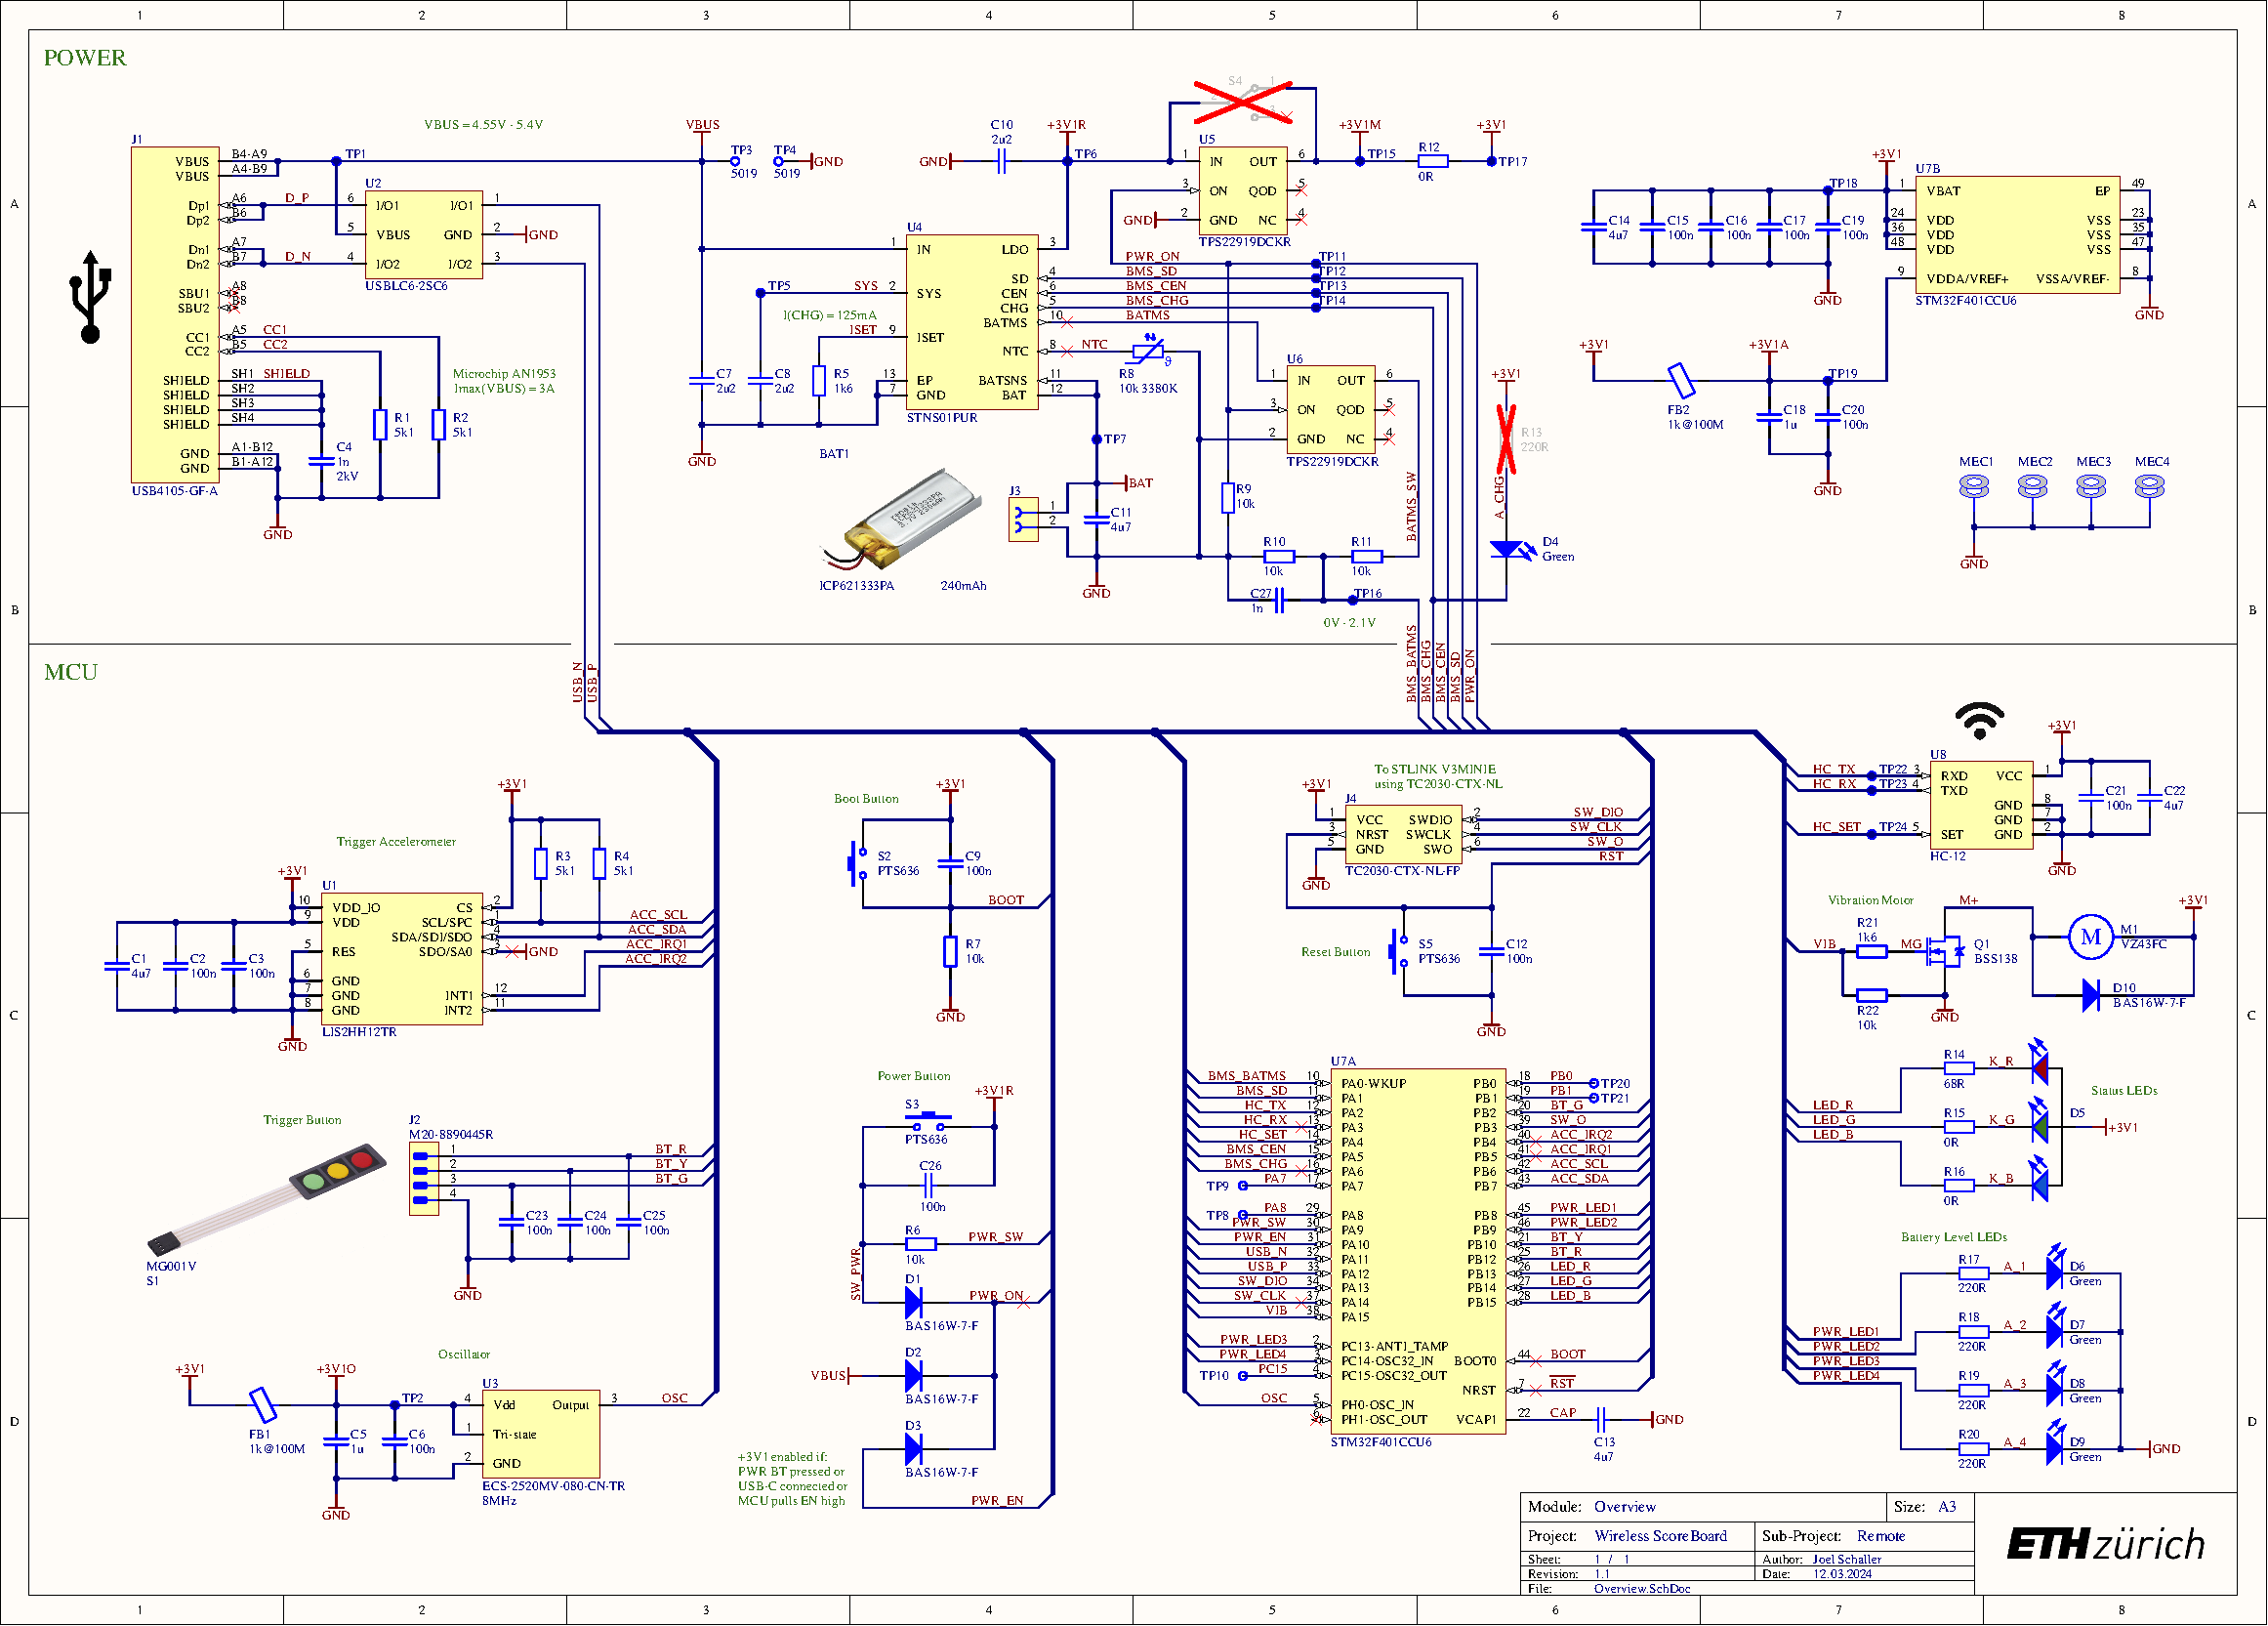
\includegraphics[width=16.7cm, trim={0.7cm 16cm 12cm 0.6cm}, clip, page=1]{../../5_Hardware/WSBR_Board/Project Outputs for WSBR_Board/WSBR_Board.PDF}}
	\caption{Battery Management Circuit}
	\label{fig:Battery Management Circuit}
\end{figure}

\subsubsection{RF module switch}
\label{sssec:RF module switch}
During the review for the WSBR Board V1.0, Mr. Malarcarne mentioned that the range of the RF Module (nRF24) could be too small to cover a whole playfield. This is due to the nRF24's frequency of 2.4GHz which allows a high data rate but much lower frequencies, than comparable modules. But for the WSB I'd need long range and a low data rate, because the remote send single byte information, of which button was pressed.

So I decided to study some alternatives with a longer range and therefore lower frequency, 433MHz or 868MHz for example \cite{RF_Modules_Comparison}. And after some research I had 2 options, either the LoRa RA-02 Module or the HC\_12 module.

\subsubsection{RA-02}
The RA-02 RF module is based on the popular SX1278 IC. This allows the RA-02 to use LoRa, a popular RF protocol used mostly for IoT applications. LoRa is optimized for use over long range with relative low data rates. The RA-02 with an antenna costs under 3 CHF on AliExpress and is also widely available on sites like DigiKey or Conrad. To communicate with the MCU, the RA-02 uses SPI and external interrupt lines, but the configuration of the module is rather complicated. But there's a library to use the RA-02 with an STM32 using HAL. But I think that the RA-02 would fit in really well, especially the design language of the WSB.
\begin{figure}[H]
	\centering
	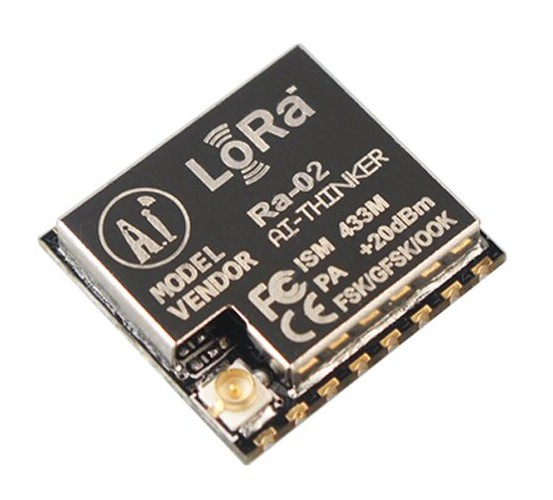
\includegraphics[width=6cm]{2_Documentation/Documentation_Wireless_ScoreBoard_Remote/Resources/RA-02.jpg}
	\caption{RF module: RA-02}
	\label{fig:RA-02}
\end{figure}

\subsubsection{HC\_12} 
The main advantage of the HC\_12 RF Module is in my opinion its simplicity. To communicate with the HC\_12 UART is used and one additional set pin. If the set pin is in the low state, the module can be configured using AT commands. There are under 10 simple commands to set the parameters such as: baud rate, transmission power, RF channel. If the set pin is in the high state, all UART packet is sent directly to the other transceiver. But on the other hand is the HC\_12 not as available online, I've bought it on AliExpress. for about 1.5 CHF. The HC\_12 has a range of up to 2km, this should be sufficient for the WSB. Because of that and its simplicity, I chose the HC\_12 for the WSB.
\cite{HC_12_doc}
\begin{figure}[H]
	\centering
	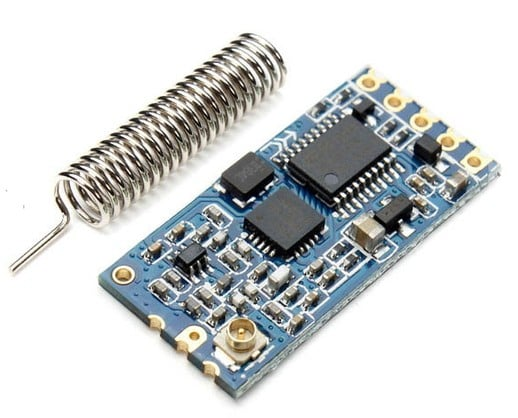
\includegraphics[width=6cm]{2_Documentation/Documentation_Wireless_ScoreBoard_Remote/Resources/HC12.jpg}
	\caption{RF module: HC\_12}
	\label{fig:HC_12}
\end{figure}

\subsubsection{Vibration Motor Decision}
\label{sssec:Vibration Motor}
Mr. Malacarne mentioned, that it would be nice to give a haptic feedback to the user of the remote. This will be achieved through a vibration motor. I personally never worked with vibration motors before, but in the past while using some devices I noticed that there are huge differences between how "good" the vibrations feel. I especially like the vibration of the iPhone, it feels expensive and of high quality. After some research, I noticed, that there are a lot of different techniques to vibrate a device. But you can sort them into two ordinate technologies. \cite{Vibration_Motors}
\begin{figure}[H]
	\centering
	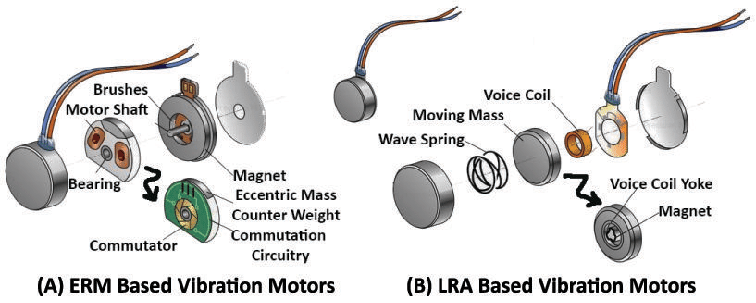
\includegraphics[width=16cm]{2_Documentation/Documentation_Wireless_ScoreBoard_Remote/Resources/ERM_LRA.png}
	\caption{Vibration motor technologies (CC NC-SA)}
	\label{fig:Vibration motor technologies}
\end{figure}

\subsubsection{ERM Vibration Motor}
Eccentric Rotating Mass vibration motors vibrate, by spinning an off-centre mass with usually a DC-motor. They can't accelerate and decelerate as fast as LRAs and don't give much control over the feel of the vibration. On the other hand, they're easy to implement, because they can just be switched on and off with an electrical switch (FET). ERM Motors shouldn't be used for direct haptic feedback such as switch mechanics simulation or tactile vibrations.

\subsubsection{LRA Vibration Motor}
Linear Resonant Actuator vibration motors on the other hand are mostly used in modern smartphones like the iPhone. They make a defined and controllable "knock" in one direction. LRAs vibrate by accelerating a mass using a magnetic field. The coils to generate this field are directly controllable with the driver circuitry. This means that an LRA has to be driven by AC (switching signal) in order to vibrate. But this allows for much more control over the feel of the vibration.

\subsection{Schematics Review}
 \label{ssec:Remote Schematics Review}
 The following changes to the project are being made after the review with Mr. Malarcarne. (Git tag before review: "WSBR/Board/V1.0")
 \begin{itemize}
     \item In the HW concept, complete the power path by feeding the signal from the load switch to board power.
     \item Add a capacitor in parallel to R10 to filter the ADC voltage.
     \item Add a vibration motor to the remote to give a haptic feedback to the user.
     \item calculate the charging time of the battery.
     \item Write chapter about RF module decision and vibration motors.
 \end{itemize}

 And check the following points:
 \begin{itemize}
     \item Alternate function mapping of the MCU.
     \item Maybe change nRF24 to another RF module with higher range (lower frequency).
     \item Accelerometer click recognition and maximum sample frequency.
 \end{itemize}

 And some further thoughts:
 \begin{itemize}
     \item The RF antenna should point away from the body into the air and should be as far as possible away from the battery.
     \item "Keep Alive" in SW and give feedback, whether the Display and remote are connected to each other and resend codes, that weren't. (ping feature)
     \item For the next time, separate signal and power hardware concepts from each other. Use the same blocks but different connection layers.
 \end{itemize}



 \subsection{PCB Assembly}
 \label{ssec:PCB Assembly}

 During the assembly of the remote PCB, I noticed a couple of possible improvements to the design.
 \begin{enumerate}
     \item The accelerometer U1 doesn't have a silkscreen, outlining its dimensions, like the BMS U4 has. During population, it was quite hard to place the accelerometer centred on the pads, due to the missing silkscreen and the pads under the IC. Next time, I would add a silkscreen to the accelerometer's footprint. 
     \item Additionally, I found out that I forgot to label the buttons (Boot, Power, Reset) on the silkscreen layer. This makes it hard for the user to use the product in the end.
     \item Add a note to the schematics with the oscillators (U2) frequency.
 \end{enumerate}

Because of the too small accelerometer, I had to install a Deadbug modification, as shown below:

 \begin{figure}[H]
	\centering
	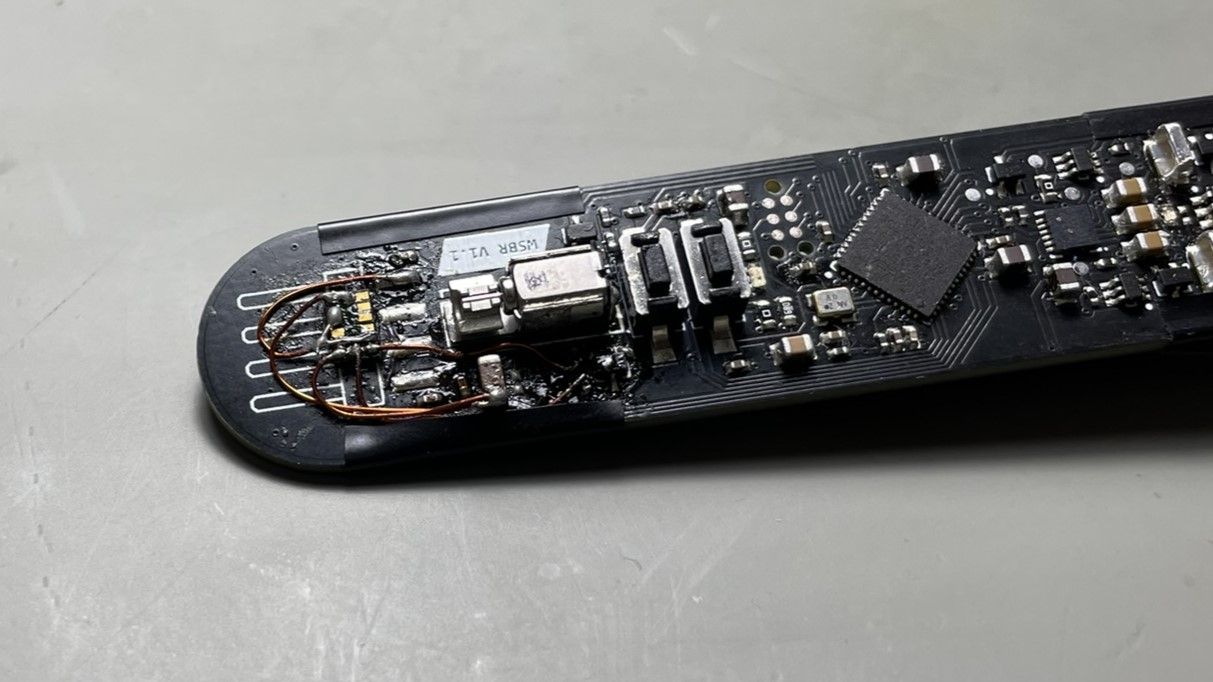
\includegraphics[width=16cm]{2_Documentation/Documentation_Wireless_ScoreBoard_Remote/Resources/IMG_1448.JPEG}
	\caption{Accelerometer Deadbug}
	\label{fig:Accelerometer Deadbug}
\end{figure}

 \section{Remote Case}

 \begin{figure}[H]
	\centering
	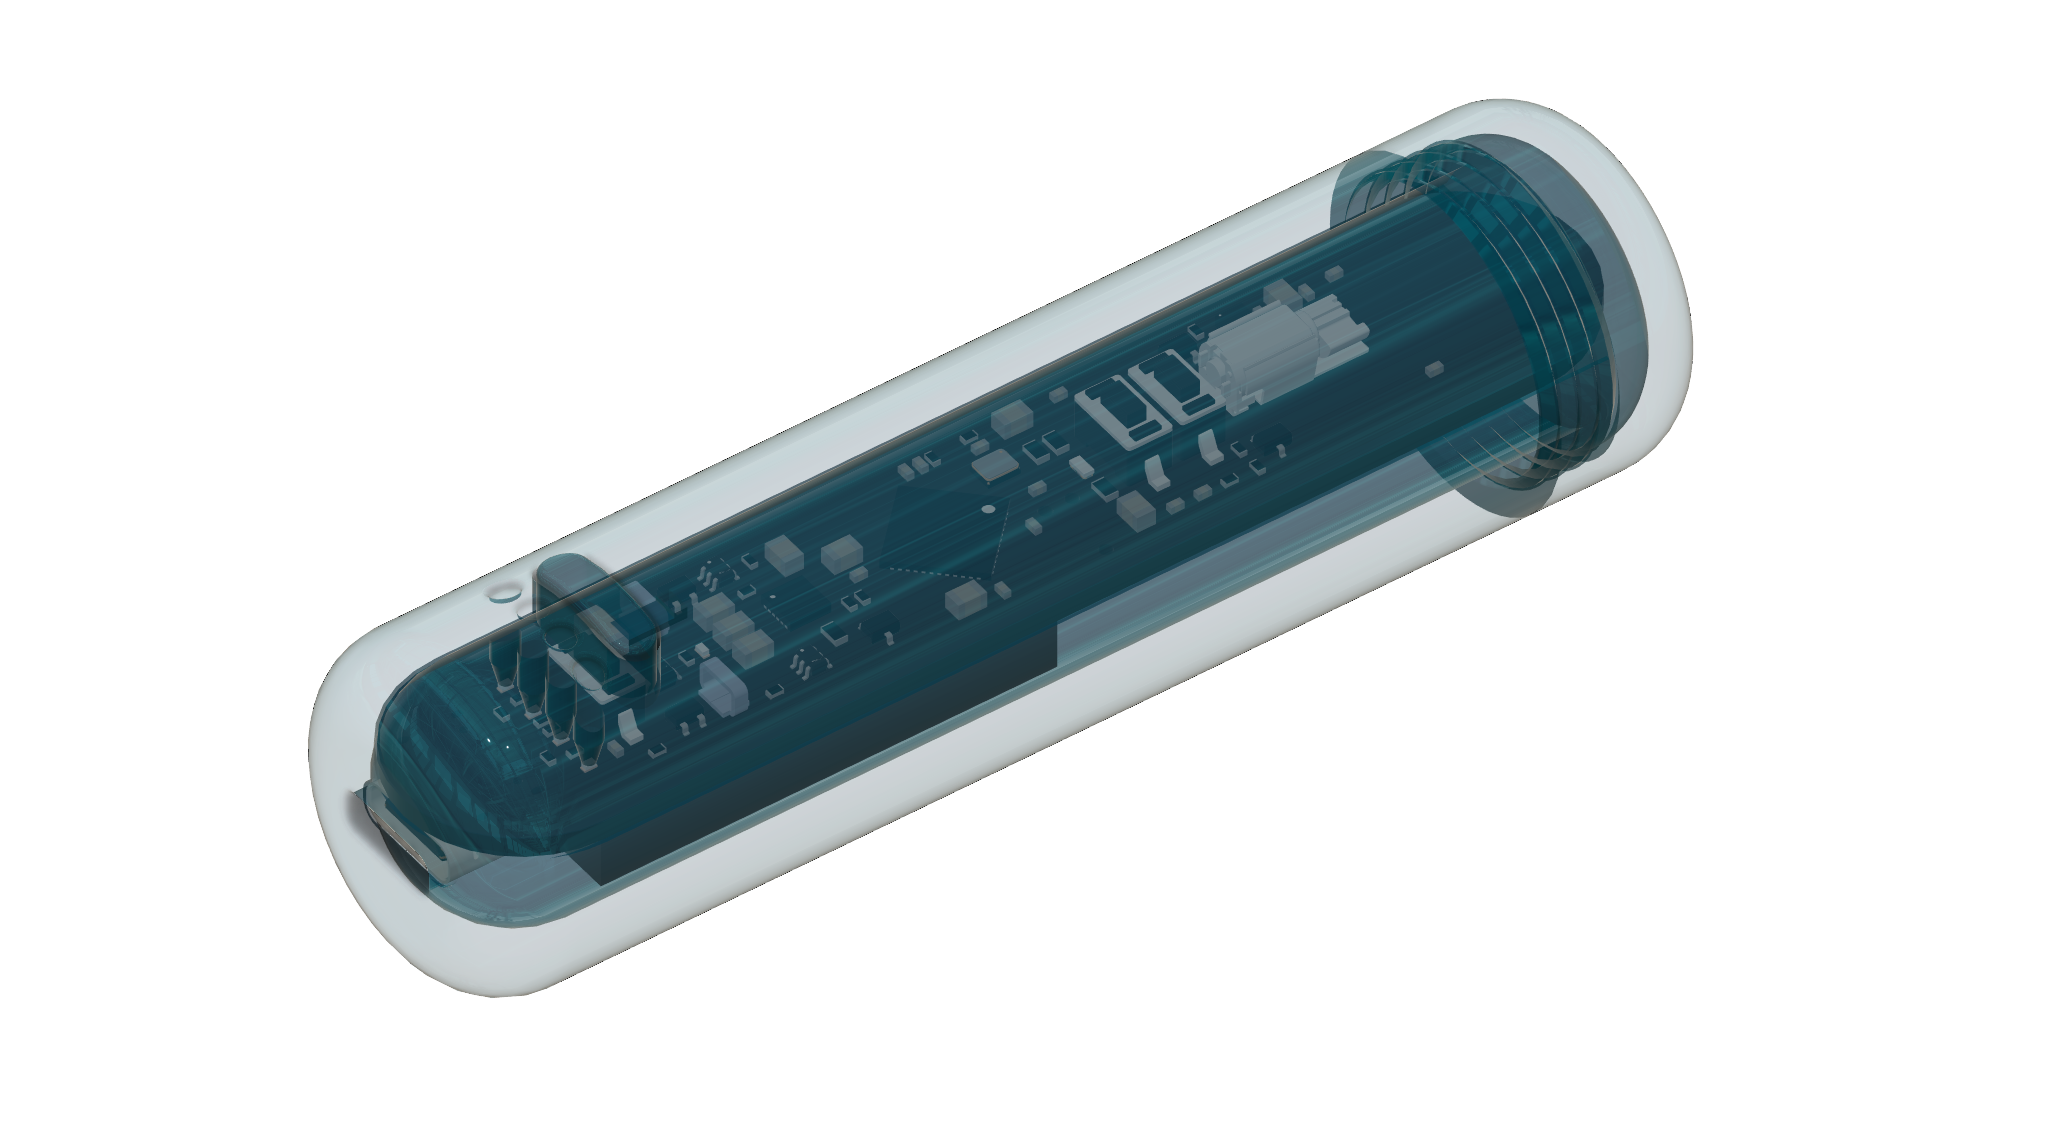
\includegraphics[width=16cm]{2_Documentation/Documentation_Wireless_ScoreBoard_Remote/Resources/WSBR_Case v8.png}
	\caption{WSBR Case Design}
	\label{fig:WSBR Case Design}
\end{figure}

I designed the Case using Fusion 360. It was my first design, including a thread. The case is divided into 2 Parts. First the tube and second the Lid. I later printed out a first prototype using my own 3d printer. While testing the tolerances for fitting the PCB into the case. The final variant of the case was manufacter by JLCPCB using a clear resin.